\documentclass{article}
\usepackage{ctex}
\usepackage{geometry}
\usepackage{amsfonts,amssymb}
\usepackage{listings} 
\usepackage{fontspec}
\usepackage{graphicx}
\geometry{a4paper,left=2.5cm,right=2.5cm,top=2cm,bottom=2cm}
\renewcommand{\baselinestretch}{1.5}
\title{科学计算作业3}	
\author{张文涛 517030910425}
\date{\today}
\lstset{columns=flexible,numbers=left,numberstyle=\tiny,basicstyle=\small,keywordstyle=\color{blue!70},commentstyle=\color{red!50!green!50!blue!50}, rulesepcolor= \color{ red!20!green!20!blue!20} }
\begin{document}
	\maketitle
	\begin{itemize}
		\item[1.]设$f(x) = a_{0} + a_{1}x + a_{2}x^{2} + \cdots + a_{n}x^{n}$,求$f[2^{0}, 2^{1}, \cdots, 2^{n}]$及$f[2^{0}, 2^{1}, \cdots, 2^{n + 1}]$。\\\\
		解:根据差商的性质,对于$n$阶可导的函数$f(x)$的任意$n$个插值节点$x_{0}, x_{1},\cdots, x_{n}$,都有
		$$f[x_{0}, x_{1}, \cdots, x_{n}] = \frac{f^{(n)}(\xi)}{n!}$$
		因此,
		$$f[2^{0}, 2^{1}, \cdots, 2^{n}] =\frac{f^{(n)}(\xi)}{n!} =a_{n}$$
		$$f[2^{0}, 2^{1}, \cdots, 2^{n+1}] =\frac{f^{(n)}(\xi)}{n!} = 0$$\\
		\item[2.]求证$n$次Newton插值基函数$\{1,(x-x_{0}), \cdots, (x - x_{0})(x - x_{1})\cdots(x - x_{n-1})\}$是线性空间$\mathbb{P}_{n}$的一组基。\\\\
		证:记$e_{0} = 1, e_{i} = (x - x_{i - 1})(1\le i\le n)$。观察到$\{1, x, x^2, x^3, \cdots, x^n\}$显然是线性空间$\mathbb{P}_{n}$的一组基。只需证明$\{e_{0},e_{1}, \cdots, e_{n}\}$可以线性表出$\{1, x, x^2, x^3, \cdots, x^n\}$即可。\\
		利用第二数学归纳法证明
		$k = 0, 1$时,有
		$$1 = e_{0}, x = e_{1} + x_{0}e_{0}$$
		由此假设当$k < p, 1 \le p \le n$时,$x^{k}$都可以被$\{e_{0},e_{1}, \cdots, e_{n}\}$线性表出,只需证明$x_{k+1}$也可以被被$\{e_{0},e_{1}, \cdots, e_{n}\}$线性表出即可。
		$$e_{k+1}=(x-x_{0})(x - x_{1})\cdots(x - x_{n-1}) \in \mathbb{P}_{k+1}$$
		故可以将$e_{k+1}$写为
		$$e_{k+1} = x^{k+1} + c_{k}x^{k} + \cdots +c_{1}x +c_{0}$$
		$$x^{k+1} =e_{k+1}  - c_{k}x^{k} - \cdots -c_{1}x -c_{0}$$
		其中$c_{i}, (0 \le i \le k)$为常数。根据归纳法假设,$x^{k}$都可以被$\{e_{0},e_{1}, \cdots, e_{n}\}$线性表出,因此证明$x_{k+1}$也可以被被$\{e_{0},e_{1}, \cdots, e_{n}\}$线性表出。所以$\{1,(x-x_{0}), \cdots, (x - x_{0})(x - x_{1})\cdots(x - x_{n-1})\}$是线性空间$\mathbb{P}_{n}$的一组基。\\
		\item[3.]设$f(x)=ln(1+x),x\in [ 0, 1],p_{n}(x)$为$f(x)$以$n+1$个等距节点$x_{i} = \frac{i}{n},i = 0, 1, 2, \cdots, n$为插值节点的$n$次插值多项式,证明:对任意$x\in [0,1]$,成立$\lim\limits_{n\rightarrow \infty} \left|f(x)-p_{n}(x)\right|=0$\\\\
		证:观察到$$\lim\limits_{n\rightarrow \infty} \left|f(x)-p_{n}(x)\right|=\lim\limits_{n\rightarrow \infty}\left|R_{n}(x)\right|$$
		并且原函数任意阶可导,因此只需要证:
		$$\lim\limits_{n\rightarrow \infty} \left|\frac{f^{(n+1)}(\xi)}{(n+1)!}x(x-\frac{1}{n})\cdots(x - 1)\right| = 0$$
		易得
		$$f^{n+1}(x) = \frac{(-1)^{n}}{(1+x)^{n+1}}$$
		所以
		$$\lim\limits_{n\rightarrow \infty} \left|\frac{f^{(n+1)}(\xi)}{(n+1)!}x(x-\frac{1}{n})\cdots(x - 1)\right| = \lim\limits_{n\rightarrow \infty}\left|\frac{(-1)^{n}}{(1+\xi)^{n+1}(n+1)!}x(x-\frac{1}{n})\cdots(x - 1)\right|$$
		并且因为$x \in [0,1]$
		$$\left| \frac{(-1)^{n}}{(1+\xi)^{n+1}(n+1)!}x(x-\frac{1}{n})\cdots(x - 1) \right| \le \left| \frac{(-1)^{n}}{(1+\xi)^{n+1}(n+1)!} \right|$$
		容易得到:
		$$\lim\limits_{n\rightarrow \infty}\left|\frac{(-1)^{n}}{(1+\xi)^{n+1}(n+1)!}\right| = 0$$
		且
		$$\left| \frac{(-1)^{n}}{(1+\xi)^{n+1}(n+1)!}x(x-\frac{1}{n})\cdots(x - 1)\right| \ge 0$$
		所以
		$$\lim\limits_{n\rightarrow \infty} \left|\frac{f^{(n+1)}(\xi)}{(n+1)!}x(x-\frac{1}{n})\cdots(x - 1)\right|=0$$
		故得证。\\
		\item[4.]设$l_{0}(x)为以节点\{x_{i}\}^{n}_{i = 0}$进行$n$次Lagrange插值相应于$x_{0}$处的基函数,证明:
		$$l_{0}(x) = 1 + \frac{x - x_{0}}{x_{0} - x_{1}} + \frac{(x - x_{0})(x-x_{1})}{(x_{0} - x_{1})(x_{0} - x_{2})} + \cdots +\frac{(x - x_{0})(x-x_{1})\cdots(x-x_{n-1})}{(x_{0} - x_{1})(x_{0} - x_{2})\cdots(x_{0} - x_{n-1})}$$.\\\\
		证:利用数学归纳法证明,进行$0$次Lagrange插值时:
		$$l_{0}(x) = 1$$
		进行$1$次Lagrange插值时:
		$$l_{0}(x) = \frac{x - x_{1}}{x_{0} - x_{1}} = 1 + \frac{x - x_{0}}{x_{0} - x_{1}}$$
		观察到等式在$n = 0,n = 1$时成立,由此假设$n = k-1$时等式成立,即:
		$$l_{0}(x) = 1 + \frac{x - x_{0}}{x_{0} - x_{1}} + \frac{(x - x_{0})(x-x_{1})}{(x_{0} - x_{1})(x_{0} - x_{2})} + \cdots +\frac{(x - x_{0})(x-x_{1})\cdots(x-x_{k-1})}{(x_{0} - x_{1})(x_{0} - x_{2})\cdots(x_{0} - x_{k-1})}=\frac{\prod_{j = 1}^{j = k - 1}(x - x_{j})}{\prod_{j = 1}^{j = k - 1}(x_{0} - x_{j})}$$
		在该等式两边加上
		$$\frac{\prod_{i = 0}^{k}(x - x_{i})}{\prod_{j = 1}^{k}(x_{0} - x_{j})}$$
		等式右边变为:
		$$\frac{\prod_{i = 1}^{k - 1}(x - x_{i})}{\prod_{j = 1}^{k}(x_{0} + x_{j})}[(x - x_{0}) +(x_{0} -x_{k})] = \frac{\prod_{i = 1}^{k}(x - x_{i})}{\prod_{j = 1}^{k}(x_{0} + x_{j})}$$
		即得到$k$次Lagrange插值下的$l_{0}(x)$,所以由归纳法,得证。\\
		\item[5.]若$f(x) = a_{0} +a_{1}x + a_{2}x^2 + \cdots + a_{n}x^{n}$有$n$个不同实根$x_{1},x_{2},\cdots, x_{n}$,证明
				$$ \sum_{j=1}\frac{x^{k}_{j}}{f'(x_{j})}=\left\{
		\begin{array}{lcl}
		0, && {0 \le k \le n - 2};\\
		\frac{1}{a_{n}}, && {k = n-1}.\\
		\end{array} \right. $$\\\\
		证:由题意得$n$次多项式$f(x)$有$n$个不同实根,由代数学基本定理可知$f(x)$可以表示为:
		$$f(x) = a_{n}(x-x_{1})(x - x_{2}) \cdots (x - x_{n})$$
		则$f'(x)$可以记为:
		$$f(x) = a_{n}\sum_{i = 1}^{n}(\prod_{k = 0, k \ne i }^{n}(x - x_{k}))$$
		则
		$$f'(x_{j}) = a_{n}\prod_{i = 0, i \ne j}^{n}(x - x_{i})$$
		可以令$p(x) = x^{k}$,则:
		$$\sum_{j=1}\frac{x^{k}_{j}}{f'(x_{j})} = \frac{p[x_{1}, x_{2}, \cdots, x_{n}]}{a_{n}} = \frac{p^{(n-1)}(\xi)}{a_{n}(n-1)!}$$
		当$k \in [0, n - 2]$时,$p^{(n-1)}(x) = 0$,\\
		当$k = n - 1$时,$p^{(n - 1)}(x) = \frac{1}{a_{n}}$,故原式得证。\\
		\item[6.]$n$次Chebyshev多项式定义为:$T_{n}(x) = \cos(n\arccos{x})$.\\
		(1)试求出$n$次Chebyshev多项式的$n$个零点.\\
		(2)设$f(x) = \frac{1}{1 + x^{2}}, x \in [-5, 5]$,以$T_{n}(x)$的零点作为插值节点,利用MATLAB分别作出$3$次Lagrange插值多项式,$6$次Lagrange插值多项式,$9$次Lagrange插值多项式,$10$次Lagrange插值多项式,并描述观察到的现象。\\\\
		(1)解:要求$T_{n}(x) = 0$,则有:
		$$n\arccos x = \frac{\pi}{2} + k\pi$$
		$$\arccos x = \frac{\pi}{2n} + \frac{k\pi}{n}$$
		$$x = \cos(\frac{\pi}{2n} + \frac{k\pi}{n})$$
		让$k$取遍$0,1,2\cdots, n-1$,则可以找到$n$个零点。\\\\
		(2)利用MATLAB,编写如下程序:
		\begin{lstlisting}[language = MATLAB]
		function yres = chebyshev(n, xres)
		k = [0:1:n-1];
		xc = cos(pi/(2*n)+k.*pi/n);
		yc = 1./(1+(xc).^2);
		res = 0;
		for i = 1 :n
		z = ones(1, length(xres));
		for j = 1:n
		if j ~= i2
		z = z.*(xres - xc(j))./(xc(i) - xc(j));
		end
		end
		res = res + z.*yc(i);
		end
		yres = res;
		plot(xres, yres);
		end
		\end{lstlisting}
		在$n$取$3, 6, 9, 10$时分别进行作图,得到如下图像:\\
		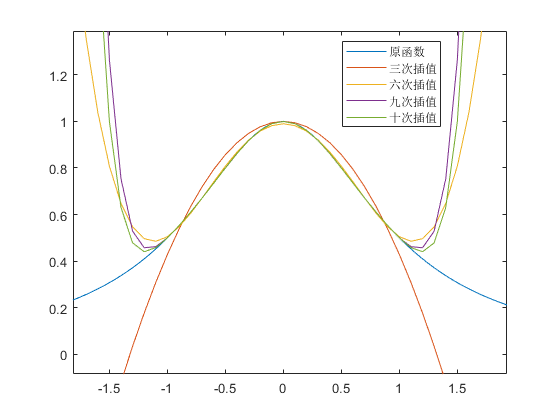
\includegraphics[scale=1]{chebyshev1.png}\\
		可以看出在Chebyshev多项式定义域内插值结果相当好,但在定义域外Runge现象非常严重。\\
		此时令$x = 5t, t \in [-1, 1]$,将函数变换到$[-1, 1]$上,将上述程序稍作修改,再取Chebyshev多项式的零点进行插值,得到如下结果。\\
		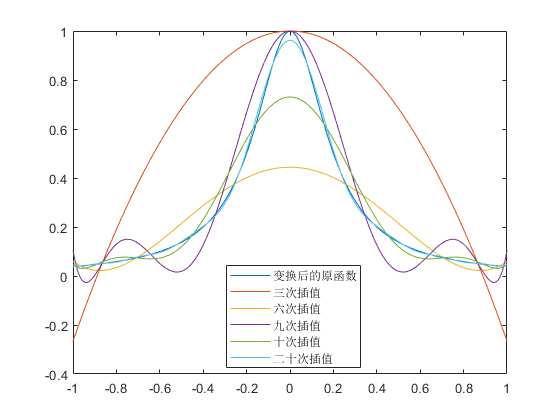
\includegraphics[scale=1]{chebyshev3.png}\\
		可以看到效果较好,并且边界处的Runge现象也消失了,达到了数值计算得到目的。	并且在尝试更高次插值时,发现插值次数增高时,插值结果变得非常好。
	\end{itemize}
\end{document}